\chapter{Testování navrženého řešení}

V předchozí kapitole byly popsány technologie, které byly v této práci použity. V této kapitole bude uvedeno několik příkladů, jak lze jednoduše vytvořit VNF v prostředí OpenStack a OpenContrail pomocí heat templatů. Všechna uvedená řešení byla testována v prostředí OpenStack s OpenContrailem, které bylo pro tyto účely poskytnuto společností tcp cloud a.s.

\section{Testovací topologie}\label{sub:interaction}

The NFV topology consist of 5 nodes. The management node is used for public IP access and is accessible via SSH. It is also used as a JUMP host to connect to all other nodes in the blueprint. The controller node is the brains of the operation and is where Openstack and OpenContrail are installed. Finally, we have three compute nodes named Compute 1, Compute 2 and Compute 3 with Nova Compute and the Opencontrail vRouter agent installed. This is where the data plane forwarding will be carried out.

The diagram below display the 5 components used in the topology. All nodes apart from the management node have 8 CPU, 16GB of RAM and 64GB of total storage. The management node has 4 CPU, 4GB of RAM and 32GB of total storage.

\begin{figure}[h]
\begin{centering}
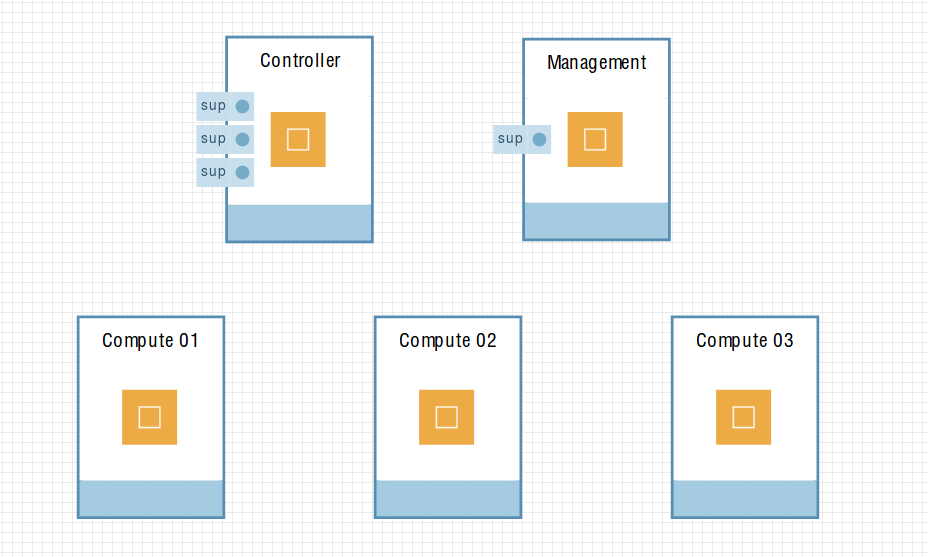
\includegraphics[scale=0.41]{images/ravello_topologie}
\par\end{centering}
\caption{Testovací topologie\label{fig:ravello_topologie}}
\end{figure}


\section{Testované síťové funkce}\label{sub:interaction}

Navrhnutá řešení v této práci předvádějí virtuální víťové funkce pro firewall a load balancing. Jsou zde ukázány celkem 3 scénáře případu užíti. Dva jsou zaměřeny na FwaaS (Firewall as a Service) a jeden na LbaaS (Load balancer as a Service). Všechna řešení jsou vytvořena pomocí Heat templatů, které se spouští v prostředí OpenStack.

Aby mohla být nějaká VNF vůbec vytvořena, tak musel být nejprve zvolen software či operační systěm, který má požadovanou funkci implementovánu. Pro tyto účely byly použity následující řešení:

\begin{itemize}
\item PFSense – open-souce firewall založený na operačním systému FreeBSD.
\item FortiGate-VM – je plnohodnotně vybavený Fortigate firewall zabalený jako virtualní instance.
\item Neutron Agent-HAproxy – je velmi rychlé a spolehlivé řešení nabízející vysokou dostupnost, load balancing a proxy pro aplikace založené na TCP a HTTP
\end{itemize}

Následující diagram znázorňuje logickou architekturu navrženého řešení dle referenční architektury zmíněné v kapitole 2.4. OpenStack spolu s OpenContrailem poskytují NFV infrastrukturu jednotlivé VNF jsou řízeny pomocí Heat.


\section{Testování LbaaS}\label{sub:interaction}

Pro vytvoření heat stacku s Load balancerem je nutné daný template vytvořit pomocí příkazu:

\verb!heat stack-create -f heat/templates/lbaas_template.hot -e heat/env/lbaas_env.env lbaas!

Tento příkaz vytvoří všechny již uvedené prostředky pro load balancing. Konkrétní load balancer má nakonfigurovanou virtual ip adresu (VIP) a k ní přiřazenou floating adresu, která je přístupná z externích sítí. Zároveň má tento load balancer přiřazený pool, ke kterému je přiřazena přiřazena privátní síť 10.10.10.0/24. Na obrázku č. X znázorňuje tento pool a obrázek č. X+1 jsou vidět členové (members) toho poolu.

\begin{figure}[h]
\begin{centering}
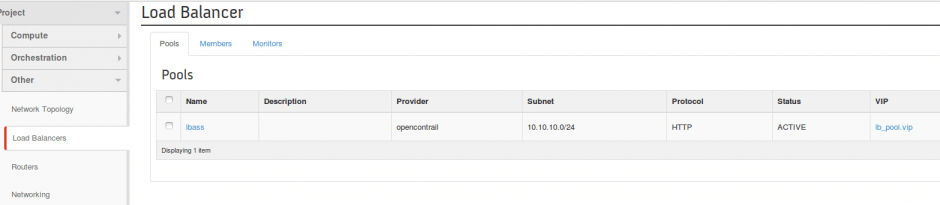
\includegraphics[scale=0.45]{images/lbaas1}
\par\end{centering}
\caption{Vytvořený pool\label{fig:lbaas1}}
\end{figure}

\begin{figure}[h]
\begin{centering}
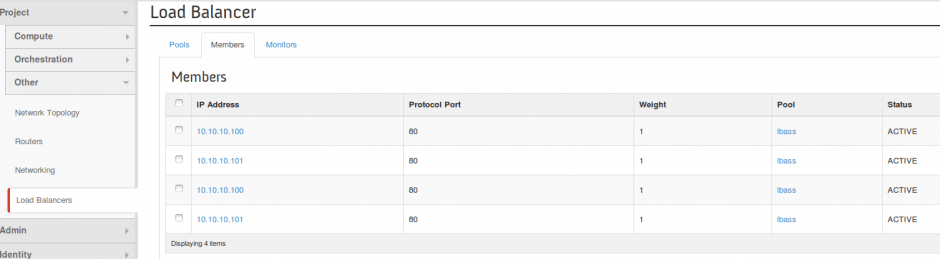
\includegraphics[scale=0.45]{images/lbaas2}
\par\end{centering}
\caption{Vytvoření members\label{fig:lbaas2}}
\end{figure}

Další zdrojem, který byl vytvořen je health monitor, který lze viděn na obrázku č. X+2. Díky němu má load balancer přehled o aktuálním stavu webových instancí. Pokud by náhodou některá z nich přestala odpovídat, v tomto případě na ping, tak by load balancer na tuto instanci přestal zasílat traffic.

\begin{figure}[h]
\begin{centering}
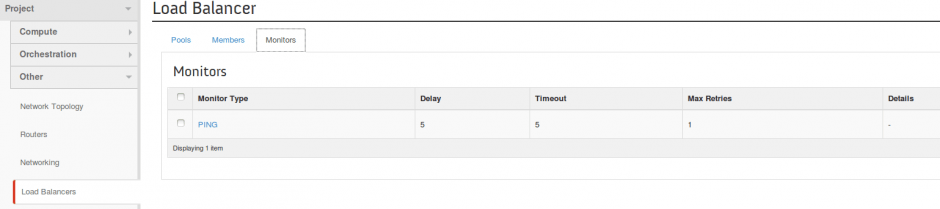
\includegraphics[scale=0.45]{images/lbaas3}
\par\end{centering}
\caption{Vytvořený health monitor\label{fig:lbaas3}}
\end{figure}

Finální síťovou topologii znázorňuje obrázek č. X+3. 


\begin{figure}[h]
\begin{centering}
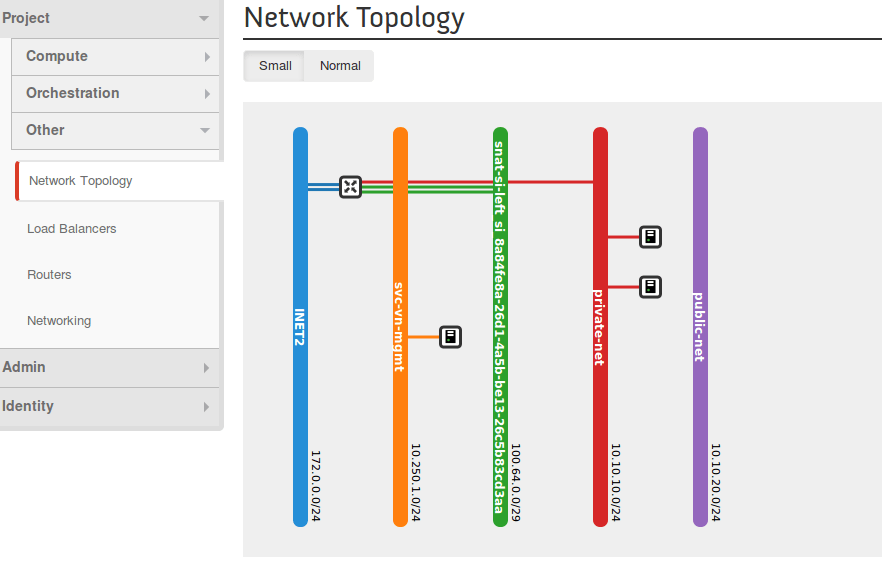
\includegraphics[scale=0.45]{images/lbaas_topologie}
\par\end{centering}
\caption{Vytvořená síťová topologie\label{fig:lbaas_topologie}}
\end{figure}

Otestování webových serverů lze provést příkazem curl, kterému dáme jako paramert ip VIP nebo floating ip load balanceru. Po několika takovýchto zadání tohoto příkazu je vidět, že oba web servery odpovídají a je probíhá mezi nimi load balancing metodou round robin.  Celý tento test je vidět na obr. č. X+4

\begin{figure}[h]
\begin{centering}
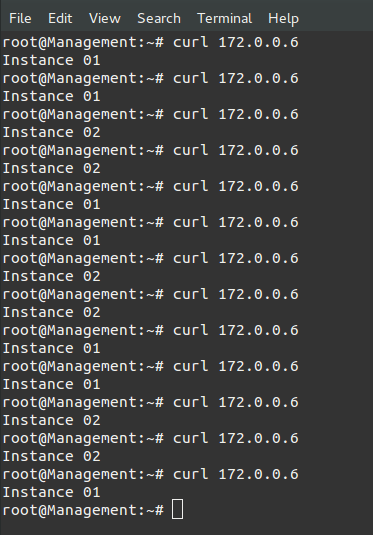
\includegraphics[scale=0.45]{images/lbaas_testing}
\par\end{centering}
\caption{Test konektivity a load balancingu\label{fig:lbaas_testing}}
\end{figure}



\section{Testování FwaaS}\label{sub:interaction}

Pro vytvoření heat stacku s PFSense z templatu lze použít příkaz:

\verb!heat stack-create -f heat/templates/fwaas_mnmg_template.hot -e heat/env/fwaas_pfsense_env.env pfsense!

a pro vytvoření heat stacku s Fortigate VM jde vytvořit pomocí příkazu:

\verb!heat stack-create -f heat/templates/fwaas_mnmg_template.hot -e heat/env/fwaas_fortios_contrail.env fortios!


\begin{figure}[h]
\begin{centering}
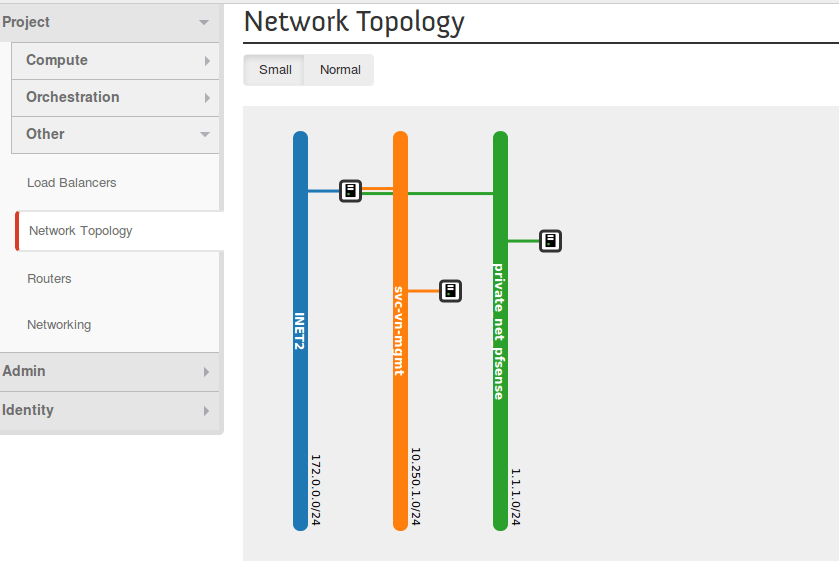
\includegraphics[scale=0.45]{images/fwaas_topologie}
\par\end{centering}
\caption{Síťová topologie\label{fig:fwaas_topologie}}
\end{figure}


By default, pfsense firewall is configured to NAT after the heat stack is started. As a result, there is no need to make any configuration for this function. Pfsense image was preconfigured with DHCP services on every interface and there is outbound policy for NAT.

After we start the heat with pfsense there is already functional service chaining. Testing instance has default gateway to contrail and contrail redirects it to pfsense.

\begin{figure}[h]
\begin{centering}
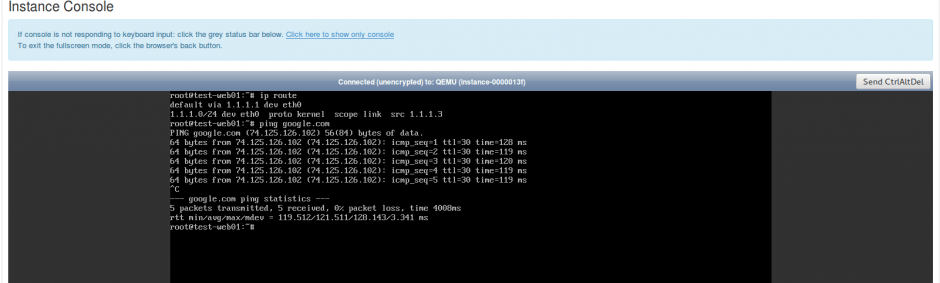
\includegraphics[scale=0.45]{images/pfsense_ping}
\par\end{centering}
\caption{Test konektivity PFSense\label{fig:pfsense_ping}}
\end{figure}

\begin{figure}[h]
\begin{centering}
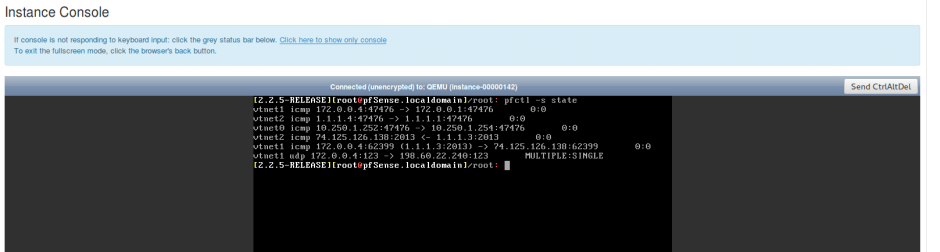
\includegraphics[scale=0.45]{images/pfsense_nat}
\par\end{centering}
\caption{Ukázka NAT session\label{fig:pfsense_nat}}
\end{figure}

There is also NAT session in pfsense. In shell run command:

\begin{figure}[h]
\begin{centering}
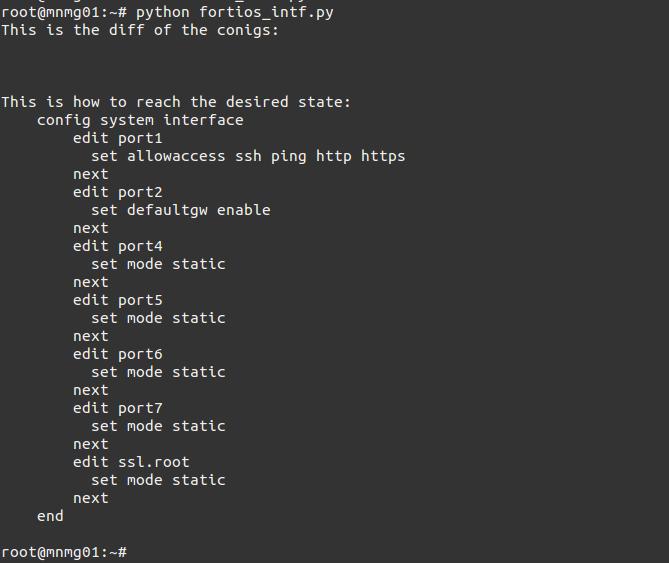
\includegraphics[scale=0.45]{images/fortigate_int}
\par\end{centering}
\caption{Fortigate VM intergace konfigurace\label{fig:fortigate_int}}
\end{figure}

\begin{figure}[h]
\begin{centering}
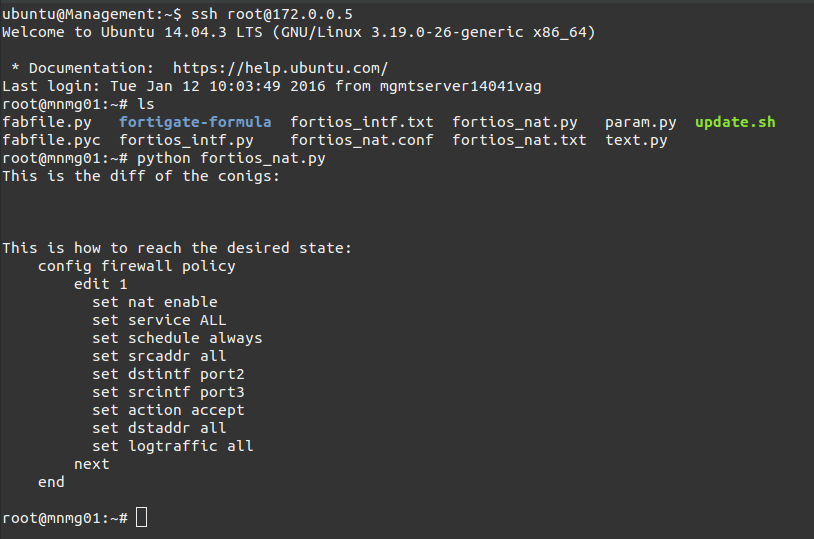
\includegraphics[scale=0.45]{images/fortigate_nat}
\par\end{centering}
\caption{Fortigate VM NAT konfigurace\label{fig:fortigate_nat}}
\end{figure}

\begin{figure}[h]
\begin{centering}
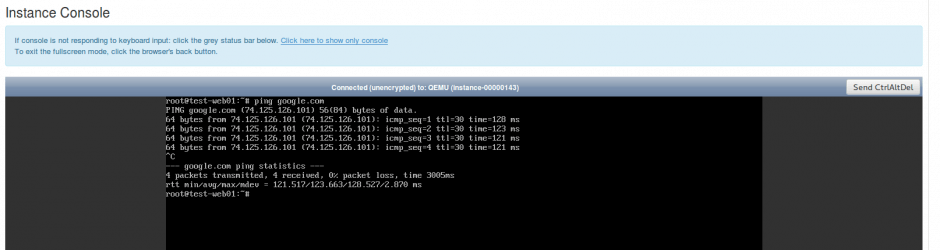
\includegraphics[scale=0.45]{images/fortigate_ping}
\par\end{centering}
\caption{Test konektivity\label{fig:fortigate_ping}}
\end{figure}


\subsection{Fortigate VM}

\subsection{PFSense}